\section{Stand der Technik / existierende Konzepte} \label{Stand der Technik}
Im folgenden Kapiel werden die einzelnen Fachsysteme der \ac{LUBW} und deren Datenbest\"ande genauer analysiert. Zus\"atzlich wird ein Blick auf das Literaturarchiv der \ac{ICT-ENSURE} gerichtet, um ein m\"oglichst \"ubergreifendes Metadatenmodell erstellen zu k\"onnen. 

Welche Metadaten die einzelnen Dokumentenbest\"ande der Fachsysteme genau enthalten, ist im Anhang \ref{Metadaten der LUBW Fachsysteme} genau aufgelistet. Hierbei wird unterschieden, ob es sich um Metadaten oder Relationen handelt. Daf\"ur wurden alle Metadaten aus den Systemen extrahiert.


Die Metadaten der in diesem Kapitel untersuchten Systeme werden anschlie\ss{}end im Kapitel \ref{Erstellung eines Datenkonzepts} zu einem \"ubergreifenden Metadatenmodell vereint, welches die sp\"atere Grundlage f\"ur die Implementierung in einem \ac{ECM}-Tool sein soll.

% Die einzelnen Fachsysteme der \ac{LUBW} sind f\"ur unterschieliche Einsatzzwecke entwickelt wurden, welche nun genauer anlaysiert werden.
% Ebenso wird das Literaturarchiv der \ac{ICT-ENSURE} untersucht, um ein \"ubergreifendes Datenmodell zu erstellen.

\subsection{FADO und Untergruppen} \label{FADO}
Das \ac{FADO}-System der \ac{LUBW} erlaubt es den Nutzern nach verschiedenen Texten aus unterschielichen Themenrichtungen zu suchen und diese herunterzuladen. Hierbei stehen die Dokumente im PDF-Format bereit.

Die einzelnen Ver\"offentlichungen k\"onnen nach verschiedenen Kriterien durchsucht werden, wobei der Bestand an Dokumenten von der \ac{LUBW} fortlaufend erweitert wird.
\cite{LUBW_FADO}

Im \ac{FADO}-System sind die Dokumente in die sechs Kategorien \texttt{Altlasten}, \texttt{Boden}, \texttt{Natur und Landschaft}, \texttt{Umweltbeobachtung}, \texttt{Umweltforschung} und \texttt{Umweltinformationssysteme} gegliedert. Hierbei ist zu beachten, dass ein Dokument nicht nur einem Themengebiet zugeordnet werden kann, sondern durchaus unter mehreren Gebieten zu finden ist. Solche Dokumente sind im \ac{FADO} jedoch nur einmal abgespeichert und werden \"uber Relationen den verschiedenen Kategorien zugeordnet.

Die einzelnen Kategorien sind wiederum mit Untergruppen versehen, welche die Zugeh\"origkeit der Dokumente konkretisieren.

Da im Verlauf der Arbeit nicht alle Gruppen in ein neues System \"uberf\"uhrt werden k\"onnen, wird sich auf die Dokumentklassen \texttt{Berichte}, \texttt{Urteile} und \texttt{Forschungsvorhaben} beschr\"ankt, welche in der Kategorie \texttt{Natur und Landschaft}, in der Kategorie \texttt{Boden} beziehungsweise in der Kategorie \texttt{Umweltforschung} zu finden sind.

Forschungsvorhaben wiederum sind Berichte, welche sich in eine Skizze, einen Zwischen- und einen Abschlussbericht aufteilen. Hierbei geh\"oren die drei Teile zu jeweils einem Forschungsvorhaben. \cite{LUBW_FADO}

\subsection{Das Document Retrieval System} \label{DRS}
Das \ac{DRS} der \ac{LUBW} ist eine Dokumentenverwaltung mit einer Art Suchmaschine, die es erm\"oglicht verschiedene Rechtsvorschriften, Regelungen, Fachberichte und Erl\"asse zu suchen. Abfragen im \ac{DRS} k\"onnen auf drei Arten erfolgen. Es gibt die "`Standardsuche"', welche es erlaubt, nach Inhalt oder Metadaten der Dokumente zu suchen. Die "`Titelsuche"' erlaubt es, wie der Name schon sagt, nach Titeln oder gegebenenfalls nach Normtiteln der Dokumente zu schauen. Als dritte M\"oglichkeit bietet das \ac{DRS} eine "`Gezielte Suche"' an, die es erm\"oglicht, Suchkriterien genau anzugeben und diese auch einzuschr\"anken.
\cite{DRS}

Zu beachten ist, dass das \ac{DRS} eine eigenst\"andiges Plattform ist, welche einen eigenen Dokumentenbestand vorh\"alt.

In Abbildung \ref{Suchmaske DRS} ist die Suchmaske der "`Gezielten Suche"' vom \ac{DRS} zu sehen. Es werden in der Maske alle M\"oglichkeiten aufgef\"uhrt, nach denen gesucht werden kann, was alle vorhandenen Metadaten mit einschlie\ss{}t. Die meisten Metadaten sind durch Auswahllisten beschr\"ankt und andere k\"onnen vom Nutzer frei mit Begriffen gef\"ullt werden.

Zu sehen ist in den Feldern \texttt{Fassung} und \texttt{\"Anderung}, dass eine Art Verwaltung von \"alteren Versionen vorgenommen wird. Diese Versionierung ist notwendig, da alte Gesetzestexte f\"ur in der Vergangenheit liegende F\"alle aufbewahrt werden m\"ussen.

\begin{figure}[!ht]
\centering
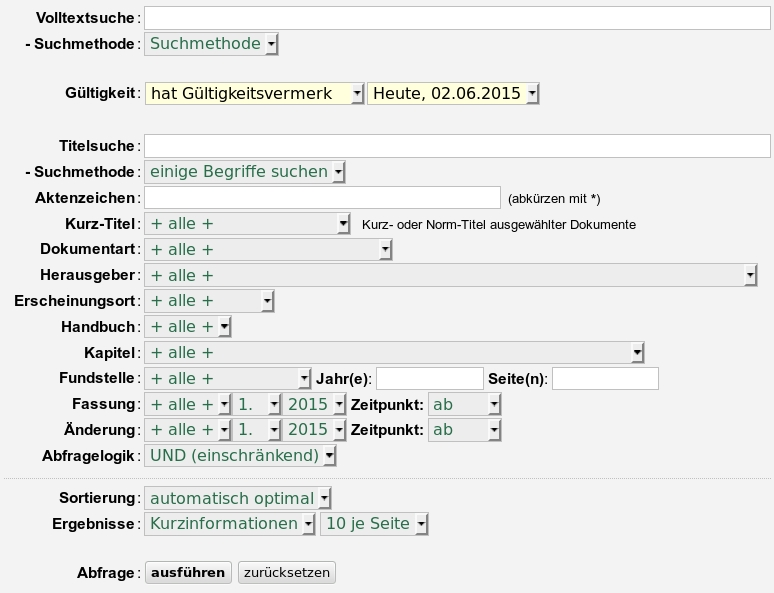
\includegraphics[width=15cm]{Bilder/Suchmaske_DRS.jpg}
\caption{Suchmaske des \ac{DRS}}
\label{Suchmaske DRS}
\centering
\end{figure}

\subsection{Naturschutz-Bildarchiv} \label{Bilddatenbank}
Im Naturschutz-Bildarchiv der \ac{LUBW} finden sich viele Bilder zu verschiedenen Themengebieten, so zum Beispiel auch zu den Gebieten \texttt{Biotoptyp}, \texttt{Lebensraumtyp}, \texttt{Naturschutzgebiet} und einige mehr.
\cite{Naturschutz-Bildarchiv}

Diese Themenkomplexe k\"onnen wiederum nach Stichworten durchsucht werden, wie zum Beispiel "`Aurorafalter"', was im Themengebiet "`Pflanzen- und Tierart"' Bilder von entsprechenden "`Faltern"' liefert. Auch das Bildarchiv ist ein eigenst\"andiges System, welches seinen eigenen Dokumentenbestand besitzt. In diesem Fall handelt es sich im Wesentlichen um Fotos.

\subsection{Literaturarchiv der ICT-ENSURE}
Im Literaturarchiv der \ac{ICT-ENSURE} sind verschiedene Dokumente zu verschiedenen Themengebieten zu finden. Die \ac{ICT-ENSURE} ist ein EU-Projekt, welches es sich zur Aufgabe gemacht hat die Zusammenarbeit von Forschung und Wissenschaft in Europa zu st\"arken.

\ac{ICT-ENSURE} enth\"alt, wie schon erw\"ahnt, viele verschiedene Dokumente aus dem Bereich Forschung und erlaubt eine Volltextsuche innerhalb dieser Dokumente. Zus\"atzlich sind die einzelnen Dokumente nach verschiedenen Fachrichtungen beziehungsweise Konferenzen gegliedert.
\cite{ICT-ENSURE_Bericht}

Im speziellen sind auf der Homepage Dokumente zu verschiedenen wissenschaftlichen Tagungen zu finden.
Alle Dokumente der \ac{ICT-ENSURE} sind B\"ucher und so erfolgt auch ihre Speicherung.
Zu jeder Konferenz gibt es ein Buch, welches in Kapitel unterteilt ist. Diese Kapitel wiederum sind in Unterkapitel geteilt, welche den einzelnen Vortr\"agen entsprechen. Jedes aufgelistete Buch entspricht einer Konferenz, die abgehalten wurde.

Eine genaue Auflistung der Metadaten ist im Anhang \ref{Metadaten der ICT-ENSURE} zu finden.
